\documentclass[17pt]{extarticle}

\usepackage[a4paper,landscape,margin=0mm]{geometry}
\usepackage{color,xcolor}
\usepackage{tikz,graphicx}

\usetikzlibrary{automata,positioning}

\usepackage{mathspec}

\setmainfont[
	Path = f/,
	BoldFont=szb.ttf,
	ItalicFont=szi.ttf,
	BoldItalicFont=szbi.ttf
		]{sz.ttf}
		
\setmathfont(Digits)[Path = f/]{sz.ttf}
\setmathfont(Latin)[Path = f/]{szi.ttf}
\setmathfont(Greek)[Path = f/, Uppercase]{g.ttf}
\setmathfont(Greek)[Path = f/, Lowercase]{g.ttf}

\setmonofont[Path = f/]{pmono.ttf}


\begin{document}

\def\hAt{-2}
\def\lAt{-3}

\definecolor{cm}{RGB}{190,0,170}
\definecolor{half}{RGB}{45,190,80}
\definecolor{each}{RGB}{215,215,215}

\def\vertgrid{
	\foreach \y in {-8,...,5} {
		\draw[color=cm,very thick] (\hAt cm - 0.8 cm,\y cm)
			node[left]{\y}
			-- (\hAt cm - 0.4 cm,\y cm);
		\foreach \t in {1,...,9} {
			\draw[color=each,thick] (\hAt cm - 0.68 cm, \y cm + 0.1*\t cm)
				-- (\hAt cm - 0.52 cm, \y cm + 0.1*\t cm);
		};
		\draw[color=half,very thick]
			(\hAt cm - 0.71 cm, \y cm + 0.5 cm)
			-- (\hAt cm - 0.49 cm, \y cm + 0.5 cm);
	};
}


\def\gorgrid{
	\foreach \y in {-11,...,11} {
		\draw[color=cm,very thick] (\y cm, \lAt cm - 0.8 cm)
			node[below]{\y}
			-- (\y cm, \lAt cm - 0.4 cm);
		\foreach \t in {1,...,9} {
			\draw[color=each,thick] (\y cm + 0.1*\t cm, \lAt cm - 0.68 cm)
				-- (\y cm + 0.1*\t cm, \lAt cm - 0.52 cm);
		};
		\draw[color=half,very thick]
			(\y cm + 0.5 cm, \lAt cm - 0.71 cm)
			-- (\y cm + 0.5 cm, \lAt cm - 0.49 cm);
	};
}



\newcommand{\restab}[3]{\begin{tabular}{ll}
	Задач решено & #1 \\
	Зачет по задачам & #2 \\
	Зачет по теории & #3 \\
\end{tabular}}

\newcommand{\certAkadem}[5]{\vfill\eject \begin{center} \tikz{
	\draw (0,0) node{\includegraphics[width=28.8cm]{o#1}};
  %	\vertgrid; \gorgrid;
	\draw (3.9,-6.1) node[right]{Золотов Б.\,А.}
	      (-2.4,-3.87) node[right]{21}
	      (-0.7,-3.87) node[right]{22}
	      (4.5,-2.6) node[right]{3.1}
	      (0,0) node{{\Large #2}}
	      (6.05,0.4) node[right]{{\footnotesize \restab{#3}{#4}{#5}}}
	      (8.1,-6.3) node{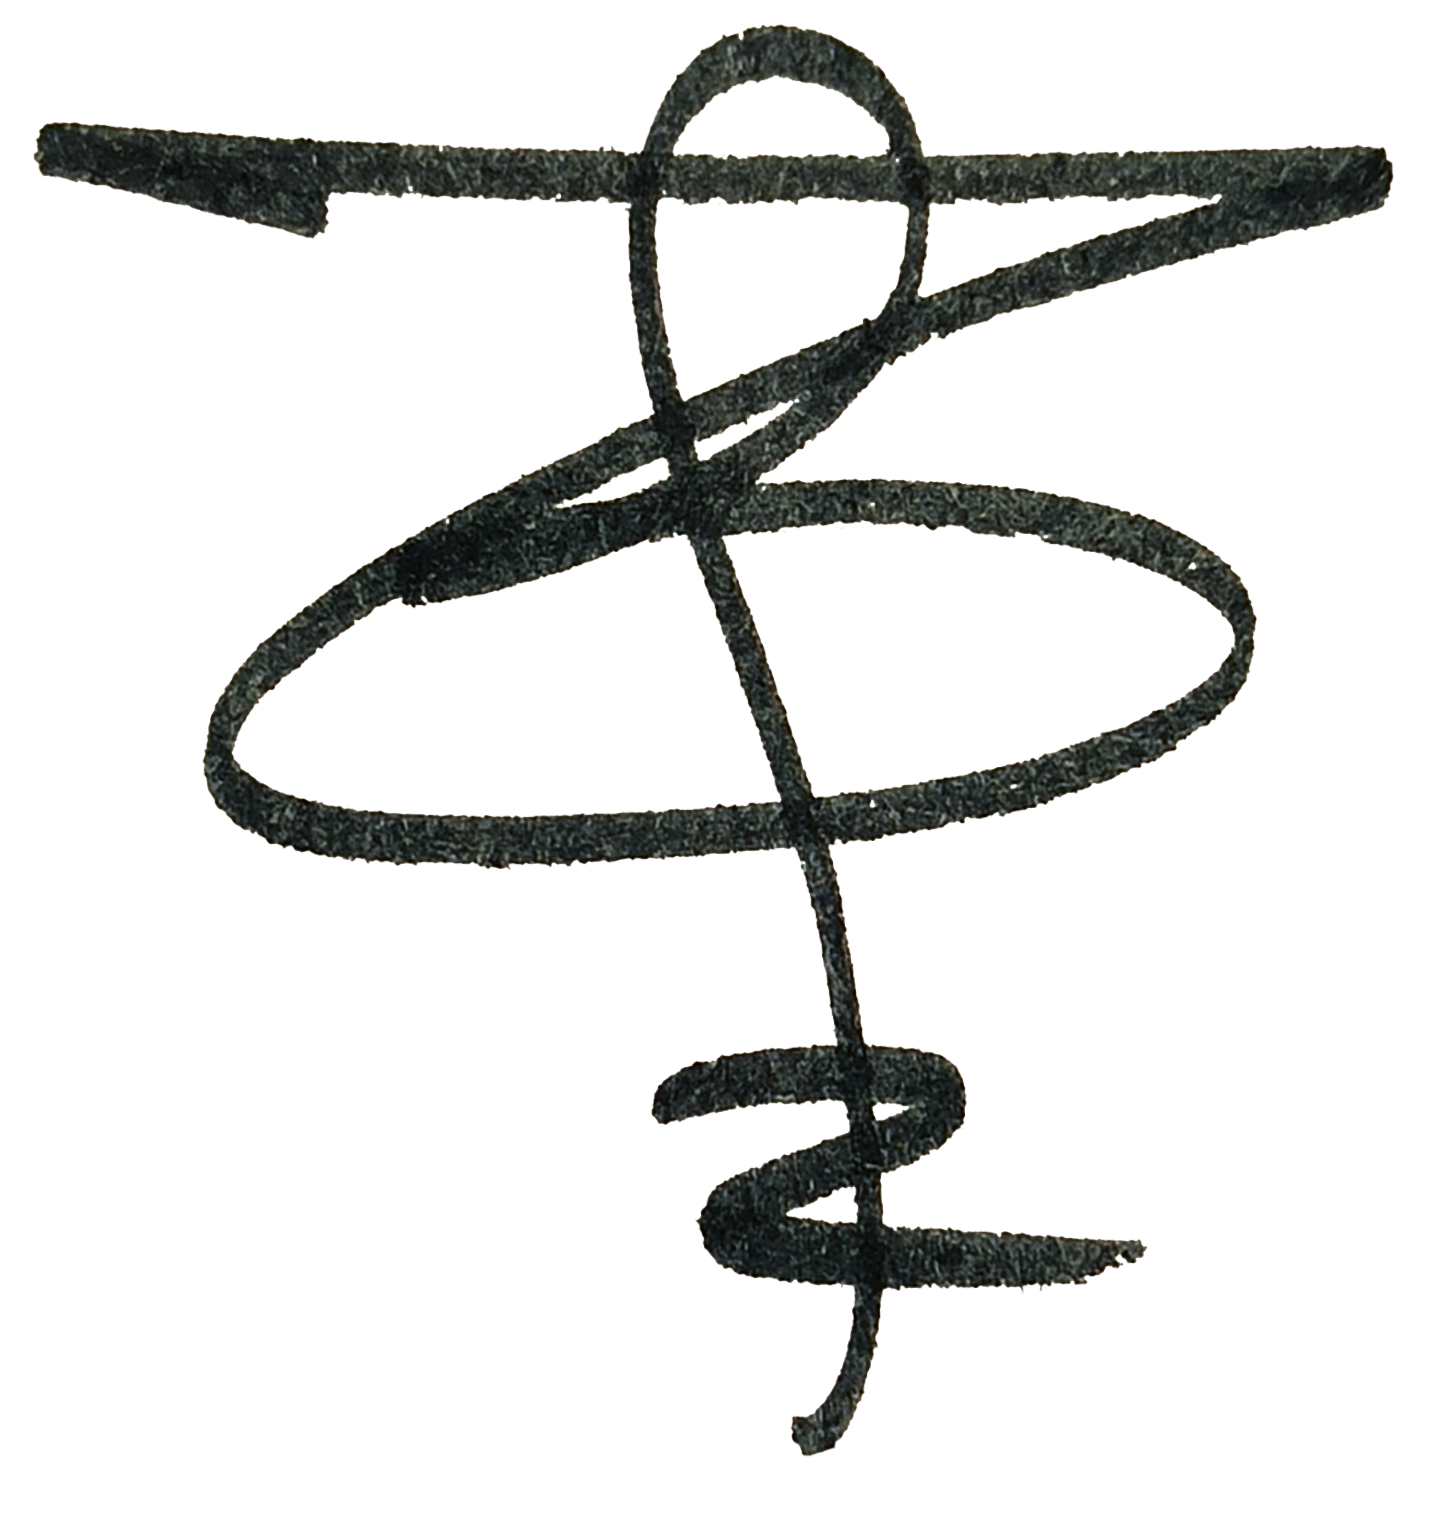
\includegraphics[height=1.7cm]{sign}};
} \end{center}}

% номер картинки, ФИО, задачи, письменно, устно

\certAkadem{3}{Виденичева Марьяна}{33,83}{3\,/\,8}{   }
\certAkadem{3}{Герасимчик Глеб}{77,5}{3\,/\,8}{   }
\certAkadem{1}{Гришин Алексей}{145}{5\,/\,8}{2,2\,/\,3}
\certAkadem{2}{Ерофеев Андрей}{71,5}{5\,/\,8}{4,5\,/\,7}
\certAkadem{2}{Самаркин Иван}{101}{5\,/\,8}{2\,/\,3}
\certAkadem{2}{Чуносов Прохор}{91,5}{4\,/\,8}{5\,/\,6}

\end{document}
